% Created 2018-10-17 Wed 18:13
% Intended LaTeX compiler: pdflatex
\documentclass[11pt]{article}
\usepackage[utf8]{inputenc}
\usepackage[T1]{fontenc}
\usepackage{graphicx}
\usepackage{grffile}
\usepackage{longtable}
\usepackage{wrapfig}
\usepackage{rotating}
\usepackage[normalem]{ulem}
\usepackage{amsmath}
\usepackage{textcomp}
\usepackage{amssymb}
\usepackage{capt-of}
\usepackage{hyperref}
\usepackage{color}
\usepackage{minted}
\usepackage{color}
\usepackage{minted}
\usepackage{parskip}
\usepackage{geometry}
\geometry{left=2.5cm,right=2.5cm,top=2.5cm,bottom=2.5cm}
\author{Daniel Moreno Manzano}
\date{\today}
\title{Ideas for future NISQ}
\hypersetup{
 pdfauthor={Daniel Moreno Manzano},
 pdftitle={Ideas for future NISQ},
 pdfkeywords={},
 pdfsubject={},
 pdfcreator={Emacs 25.1.1 (Org mode 9.0.5)}, 
 pdflang={English}}
\begin{document}

\maketitle

\section{Portals}
\label{sec:org995b045}

\subsection{Introduction}
\label{sec:org3d38321}

The two main advantages -- and the basis of the computational power -- of the quantum computers are the superposition and entanglement phenomena.
Based on those, the teleportation of information is possible.

A bit far from that promising context with high computation power, in the NISQ era, the real devices are highly constrained and with low amount of qubits. 
The most common constraint is the Nearest Neighbor one.
Except for some technologies like Ion Traps, most of the devices need to arrange the qubits in a mesh layout.
Therefore, a mapping process that initiates the qubits in the best possible place and routes them is needed.

In the future NISQ era, with computer of hundreds of qubits, a fast way of moving the qubits to far places is required.
Taking into account the Nearest Neighbor constraint and the teleportation ability of quantum devices, the idea of arranging special teleportation regions pops up.
I call \emph{portals} to this regions.

\subsection{Main idea}
\label{sec:orga729753}

As explained before, the future NISQ era needs a faster way to move the qubits around than the SWAP method.
With \emph{portals} in strategic places in the quantum chip, the qubits will be able to transmit their states efficiently and faster than using the SWAP method.

\subsubsection{Steps}
\label{sec:org01ff635}

The steps that this method requires are:

\begin{enumerate}
\item EPR pair generation and distribution
\item SWAP between the state we want to transmit and the closest EPR qubit (portal)
\item Apply the first part of the teleportation circuit between the source qubit and one of the EPR qubits
\item Measure and store the result in a classical register
\item Apply the last part of the teleportation circuit to the target qubit
\end{enumerate}


\subsubsection{Pros and cons}
\label{sec:org1aeddfa}

Some of the drawbacks and advantages are:

\begin{table}[htbp]
\centering
\begin{tabular}{ll}
\uline{Cons} & \uline{Pros}\\
 & \\
 & \\
- Long time of measuring & - Is efficient for distances greater than 6 qubits (fig. \ref{fig:org55aa851})\\
- Difficulty of EPR pair generation & - Circuit/purpose specific chips could be optimized\\
- Classical registers required & \\
\end{tabular}
\end{table}


\begin{figure}[htbp]
\centering
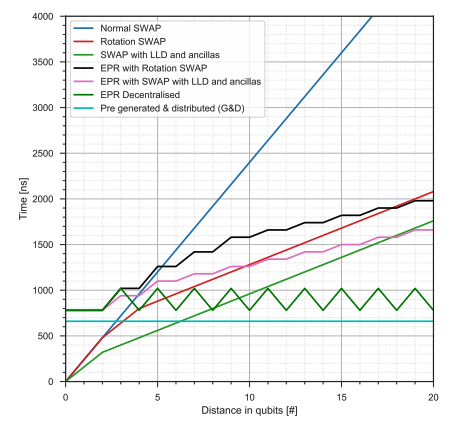
\includegraphics[width=0.5\textwidth]{total_exec_t_transp_methods.png}
\caption{\label{fig:org55aa851}
Execution time for several transportation methods from Bas thesis}
\end{figure}

\subsubsection{Instance}
\label{sec:org287e669}

E.g. assuming and infinit grid of qubits with a region highly congested -- an area with all the qubits constantly in use -- the computation requires the route of some qubit to another specific place.
In order to depict a difficult scenario, one can see, in fig. \ref{fig:org5b810a8}, that the congested area is between the origin and final position of the yellow qubit -- the one that needs to be routed.
Using the SWAP method to route the qubit state will result in a long path, in order to avoid the congested area.

\begin{figure}[htbp]
\centering
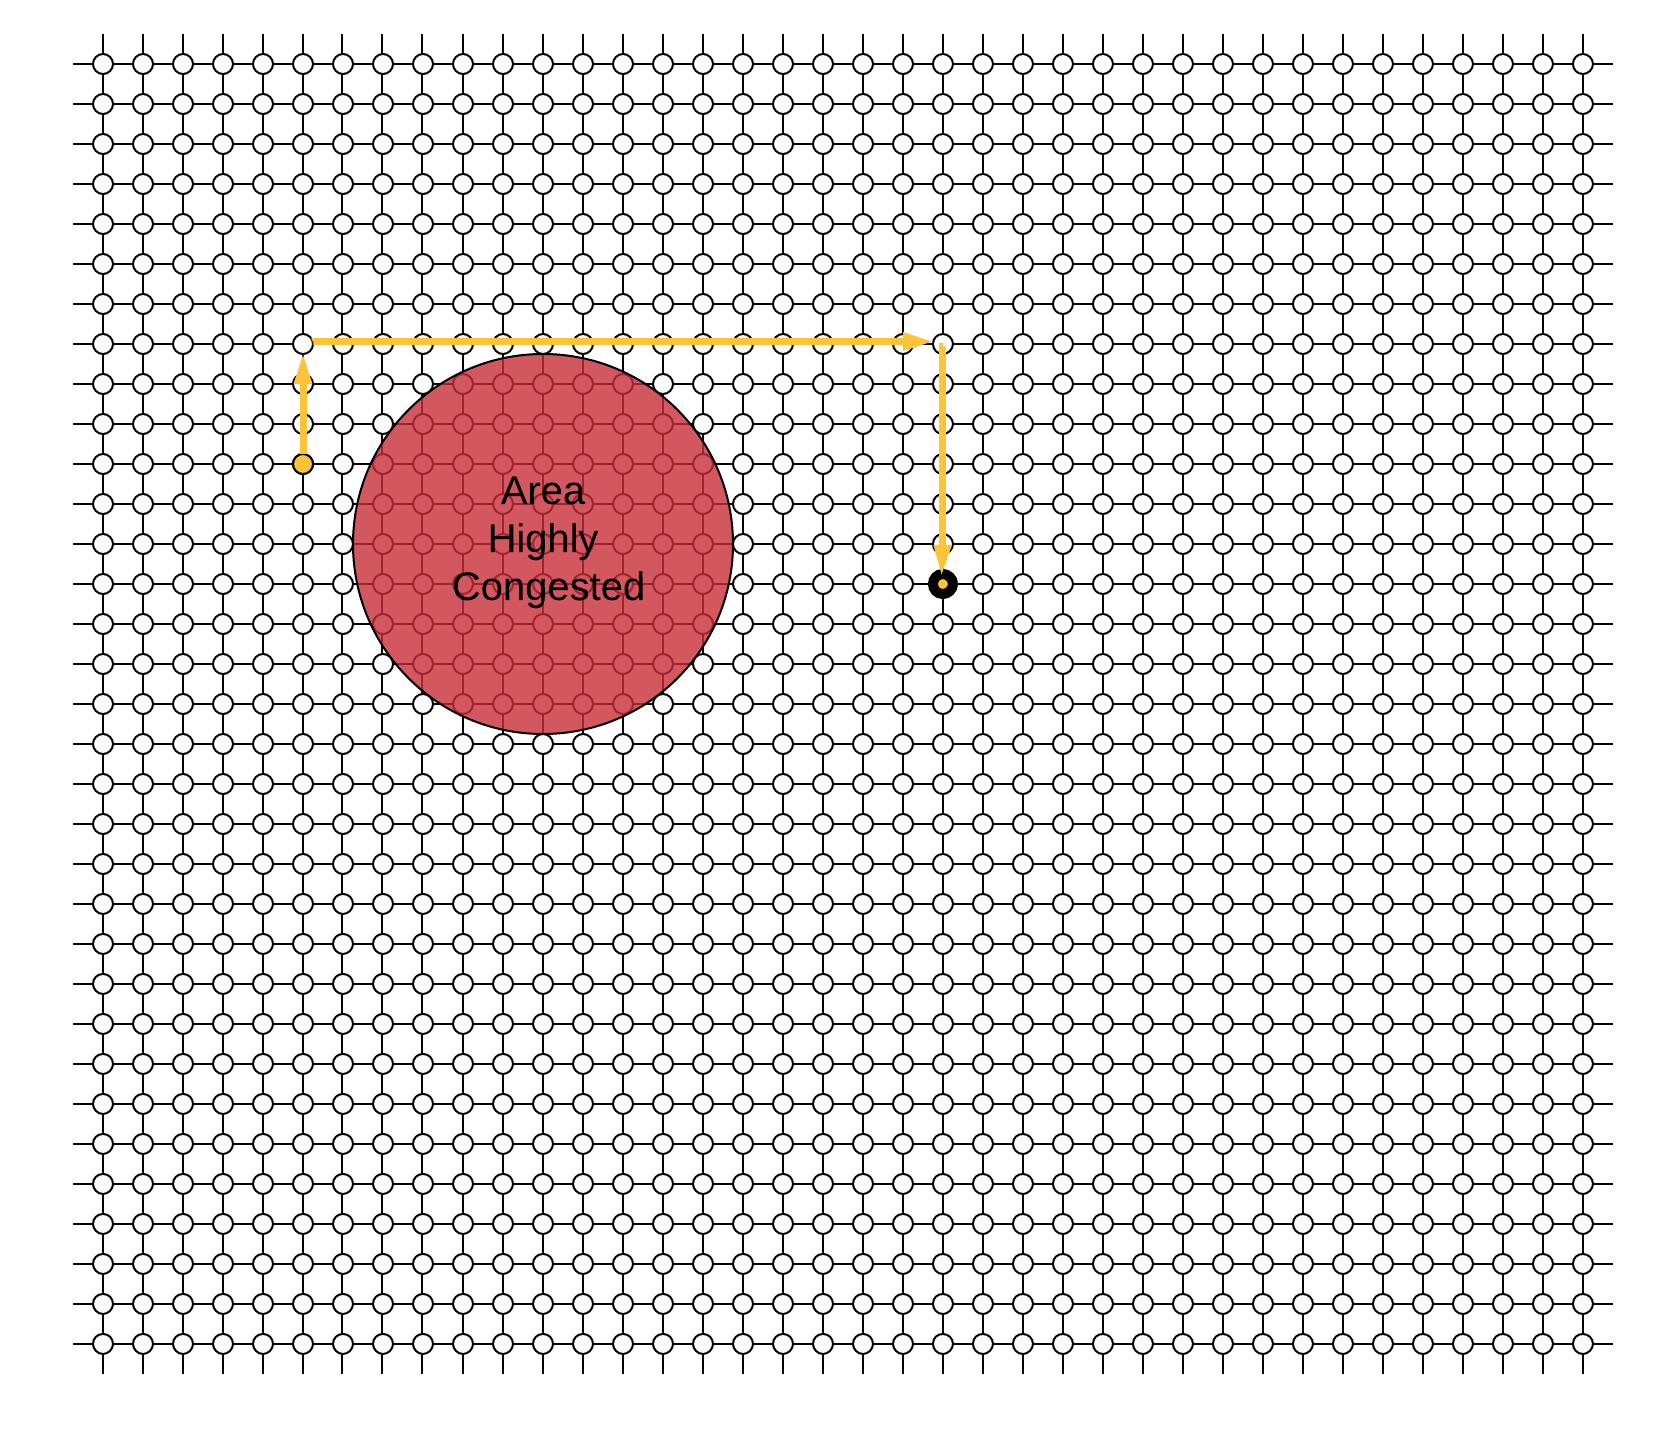
\includegraphics[width=\textwidth]{Teletransmission1.png}
\caption{\label{fig:org5b810a8}
Example of the movement required for a qubit based on SWAP in the context of a highly congested region in between}
\end{figure}

On the other hand, using the teleportation method, the path shortens a lot as one can see in fig. \ref{fig:org167b470}.

\begin{figure}[htbp]
\centering
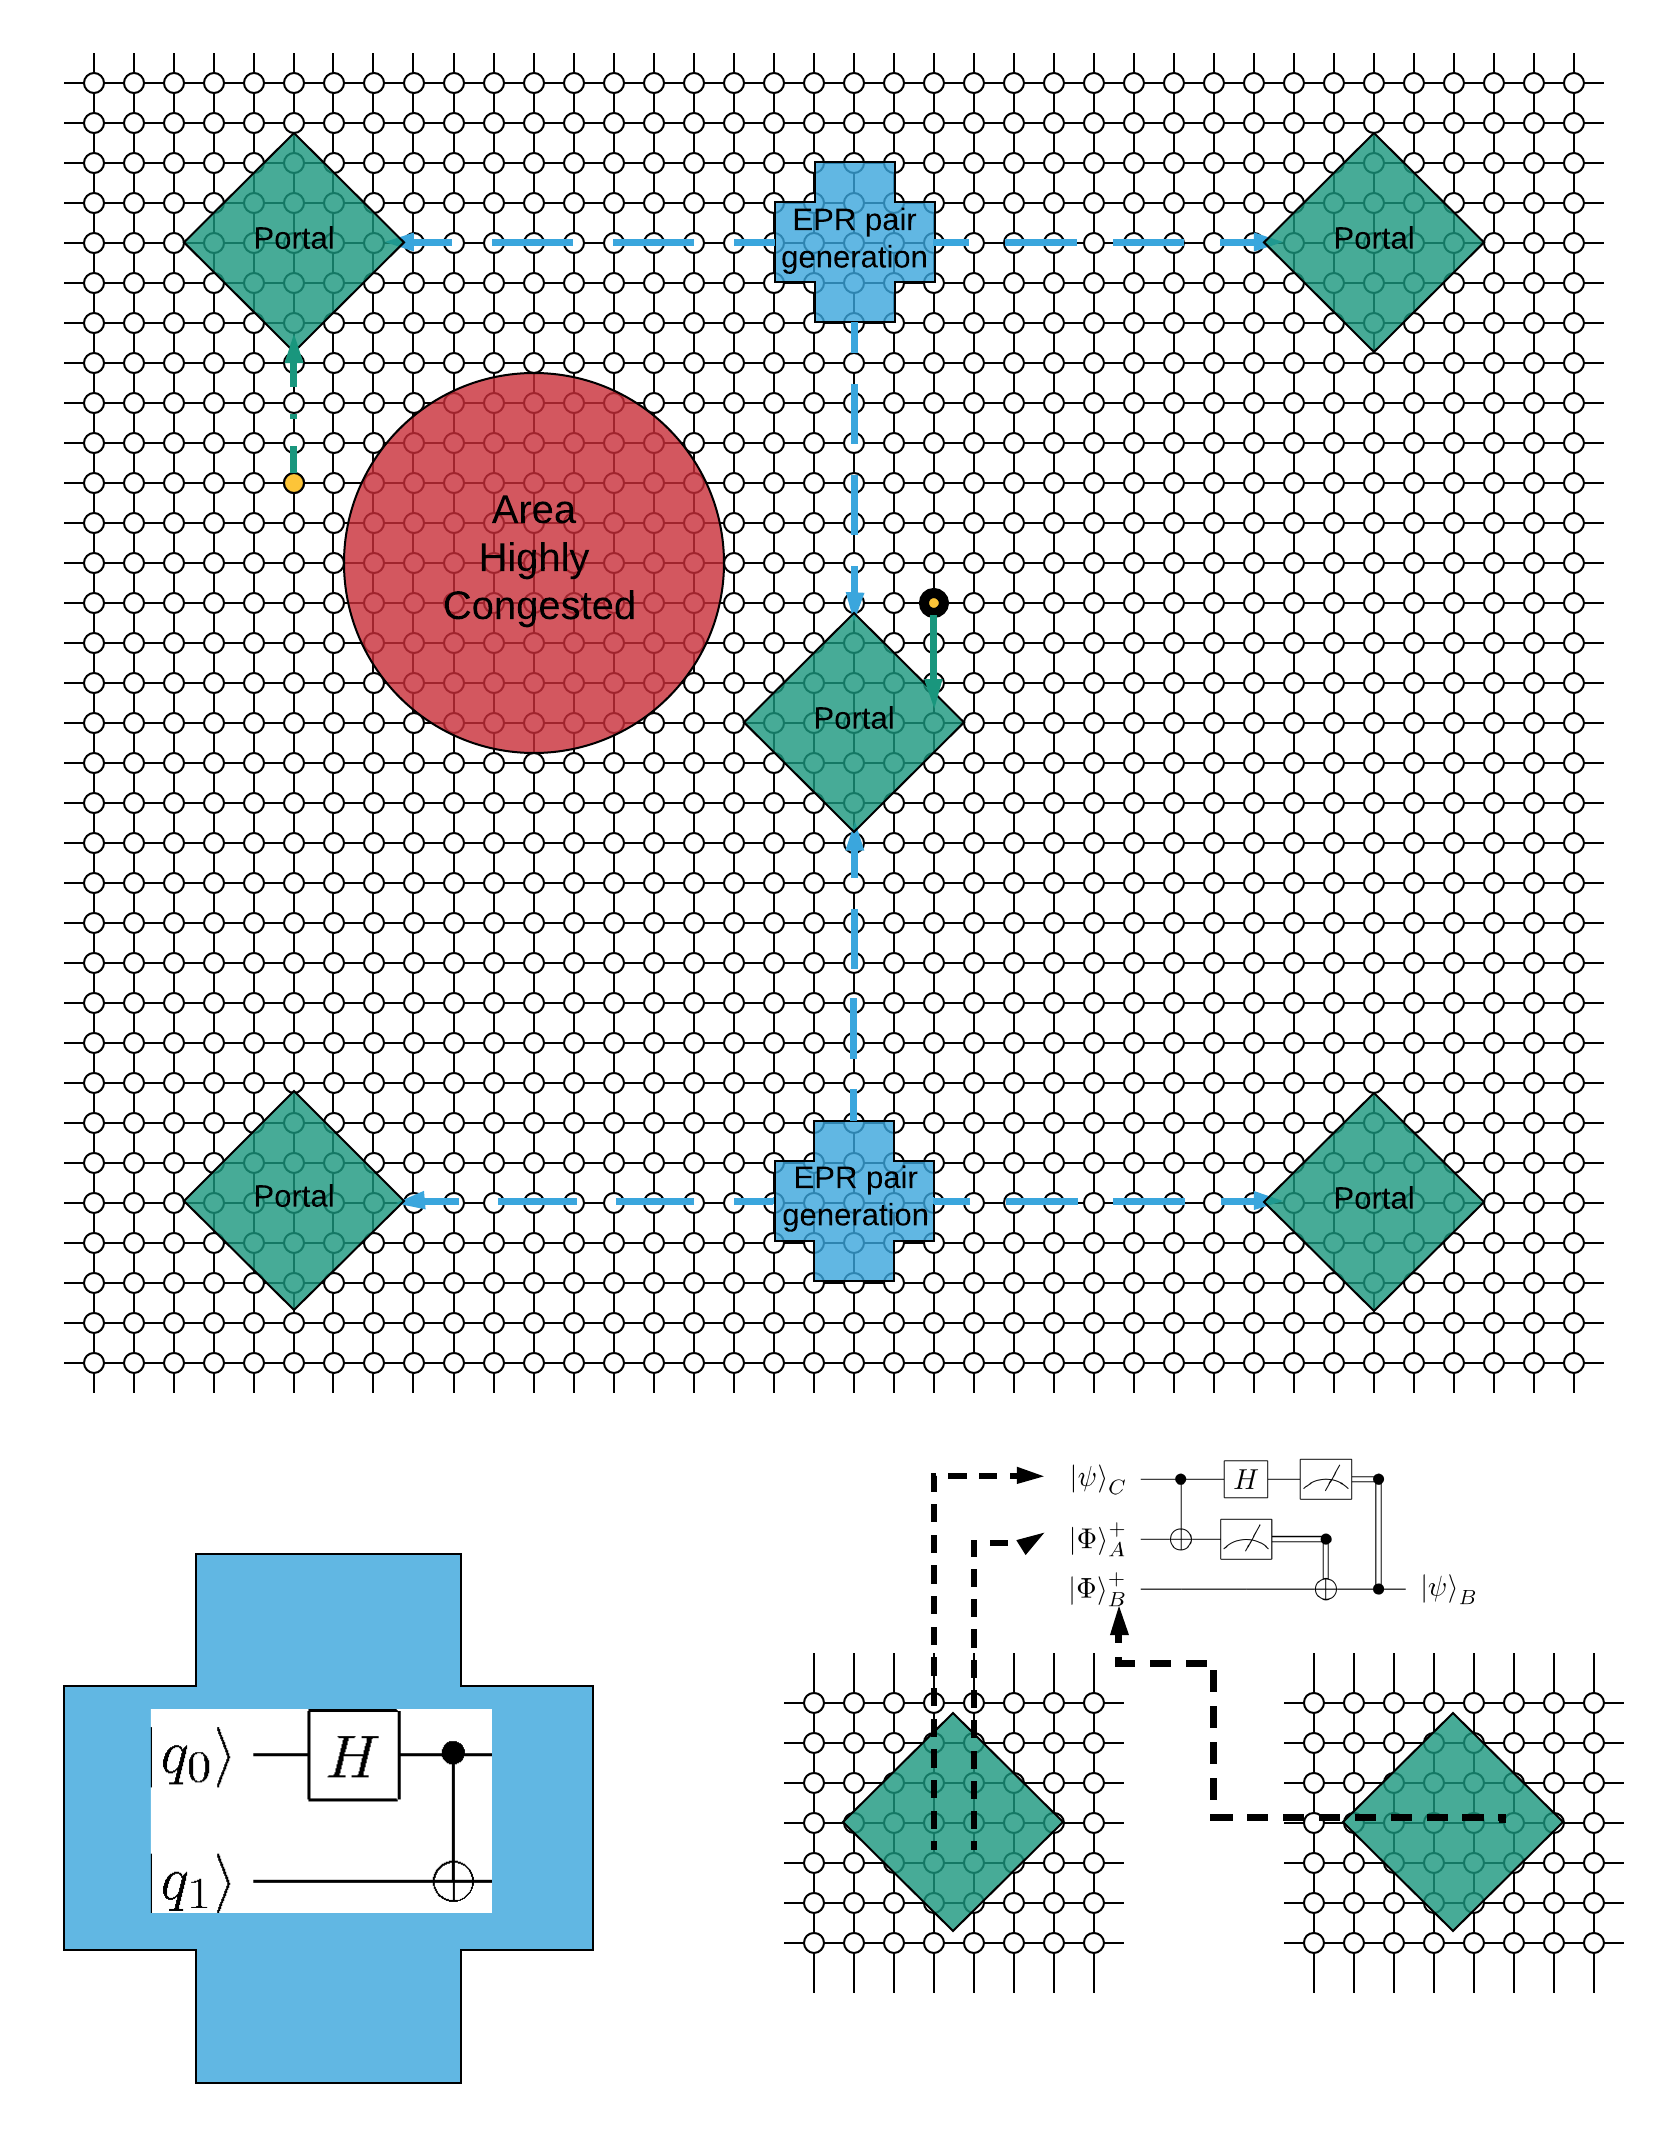
\includegraphics[width=\textwidth]{Teletransmission2.png}
\caption{\label{fig:org167b470}
Specification and example of the movement required for a qubit based on teleportation methods in the context of a highly congested region in between}
\end{figure}
\end{document}
